%!TEX root = ../Main.tex
\label{sec:actors}

I dette afsnit beskrives aktører og deres rolle i systemet. I figur~\ref{fig:actordiagram} ses aktørdiagrammet, som beskriver alle aktører og deres forhold til systemet.
\begin{figure}[H]
	\centering
	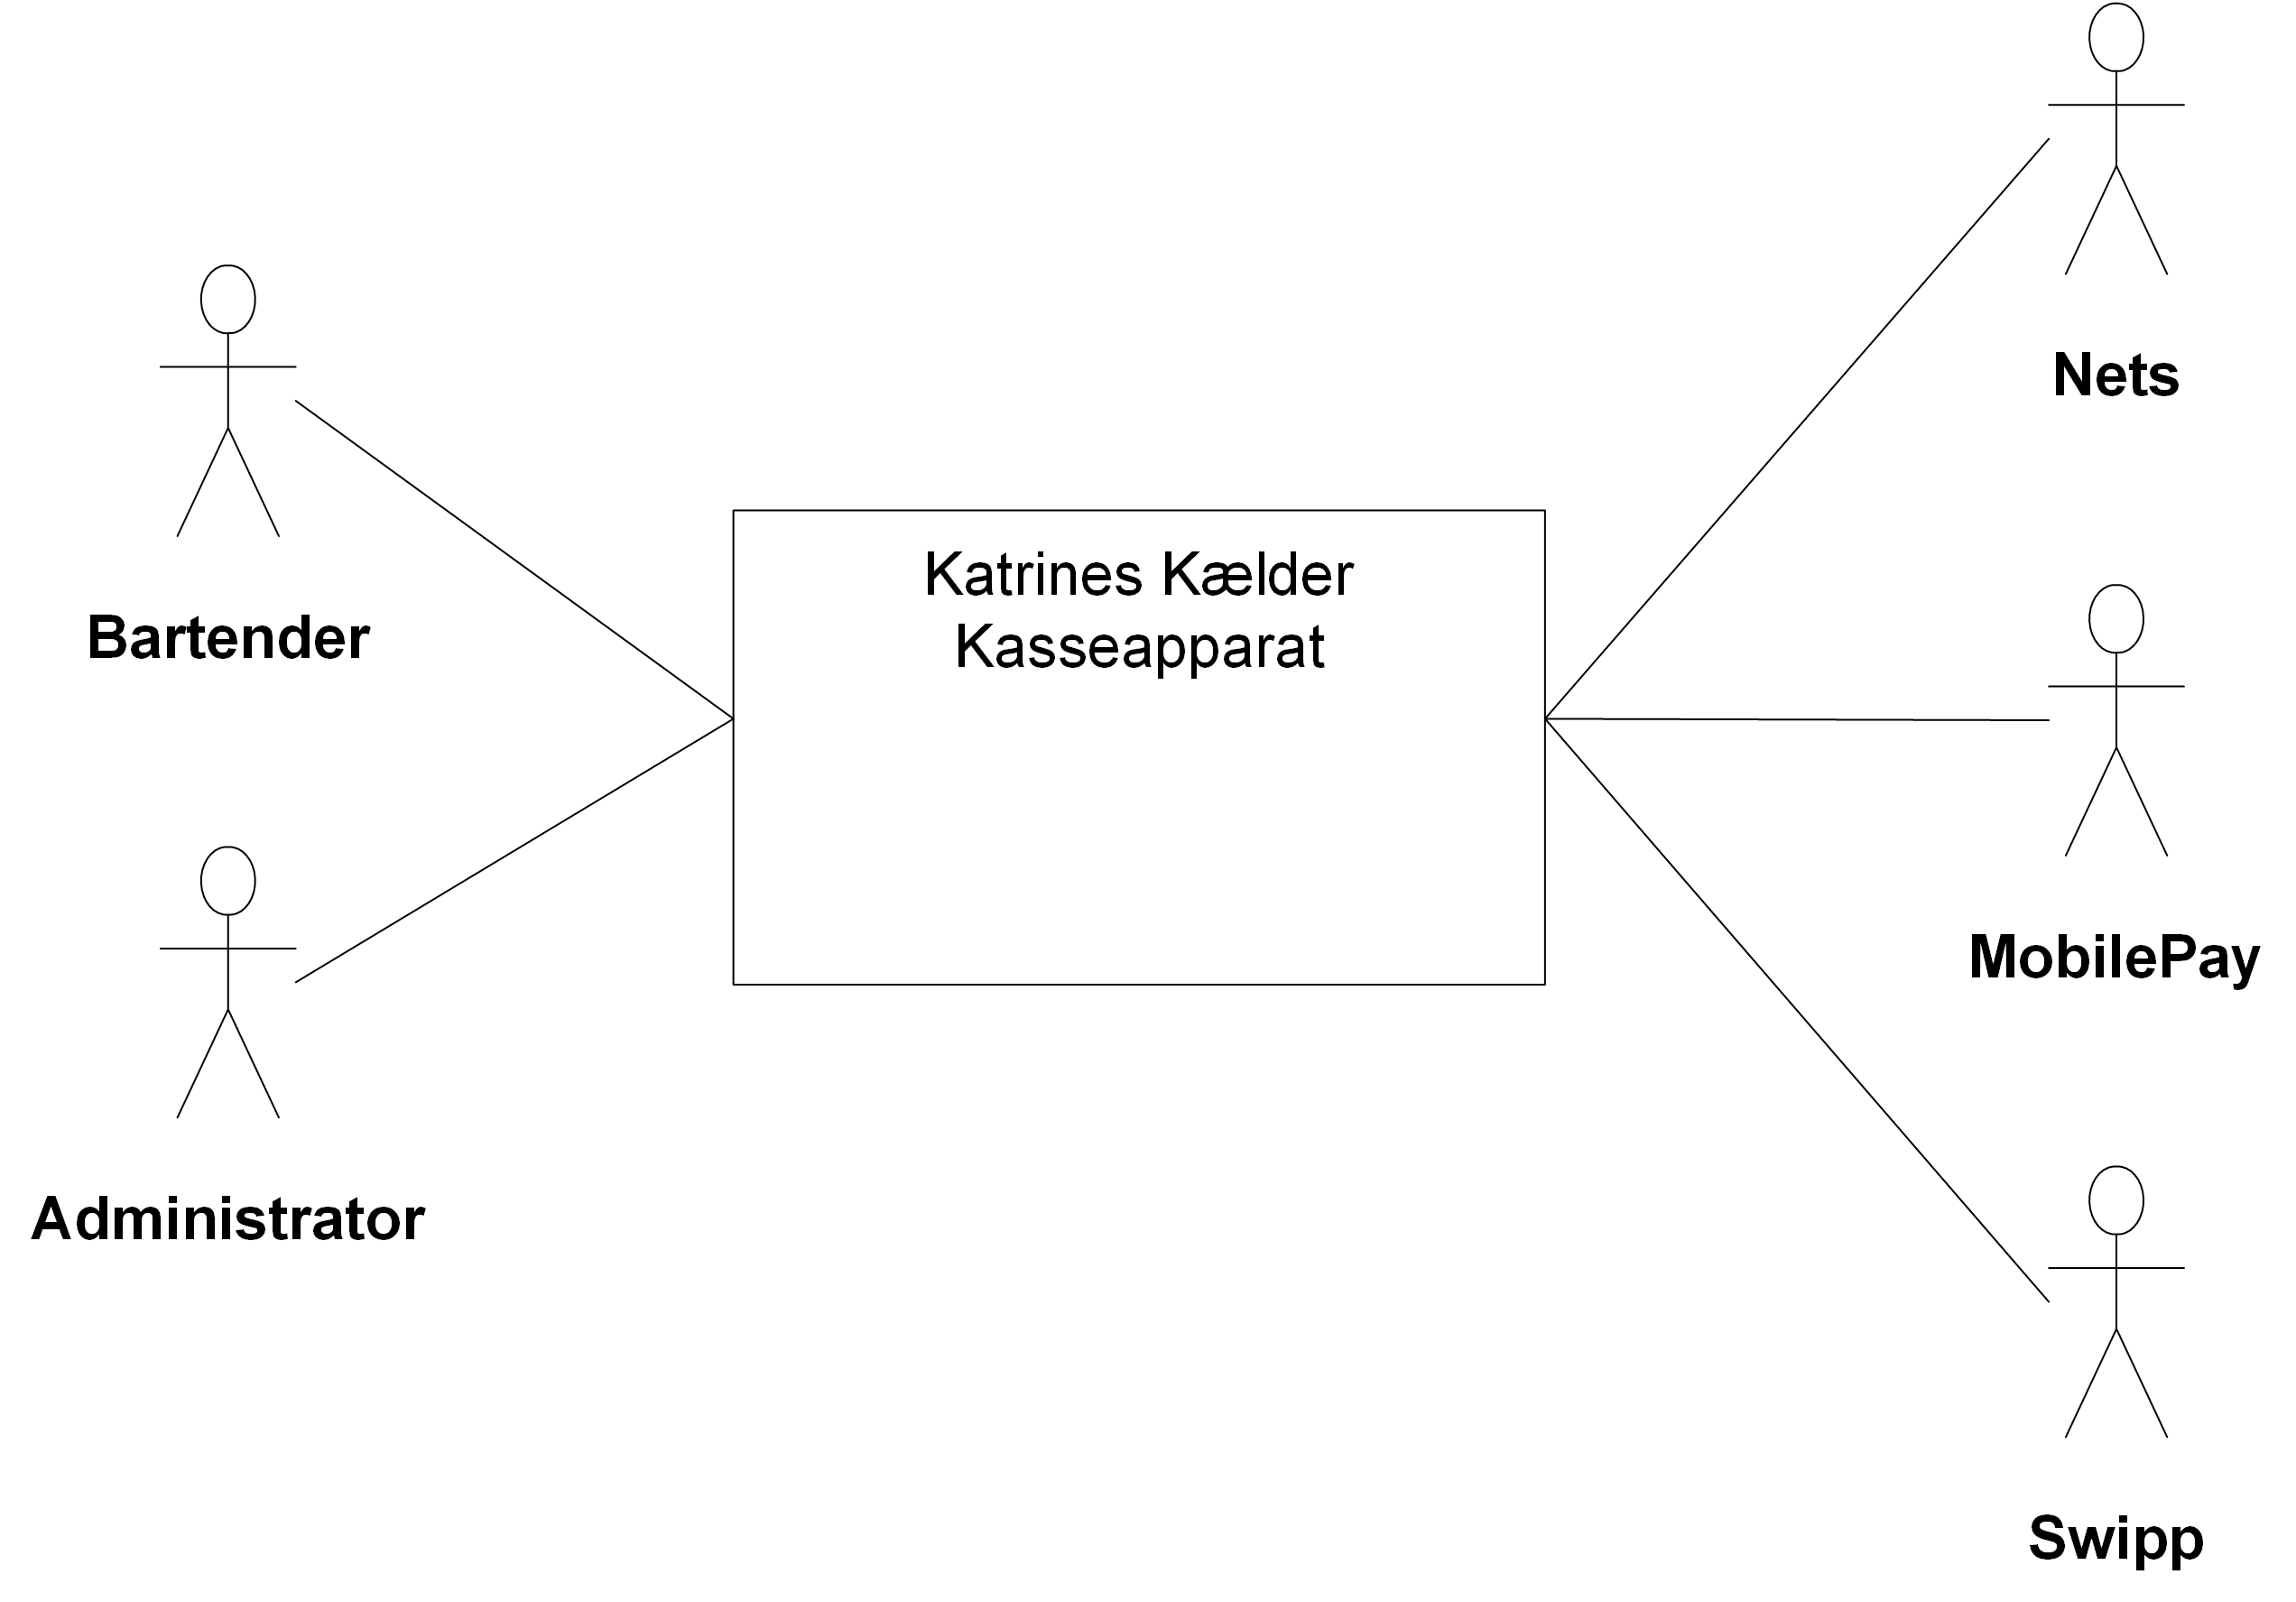
\includegraphics[width=0.8\textwidth]{Kravspecifikation/Actor/Actor.png}
	\caption{Aktør-kontekst diagram}
	\label{fig:actordiagram}
\end{figure}

\newpage
\begin{actor}{Bartender}
\field{Type:}{Primær}
\field{Beskrivelse:}{\textit{Bartender} er den primære bruger af systemet, og står for salg af varer.}
\end{actor}

\begin{actor}{Administrator}
\field{Type:}{Primær}
\field{Beskrivelse:}{\Gls{administrator} skal stå for logistikken (priser, varelager osv.) gennem systemet.}
\end{actor}

\begin{actor}{Nets}
\field{Type:}{Sekundær}
\field{Beskrivelse:}{\textit{Nets} er leverandøren af betalingsterminalen. Betalingsløsningen er en af systemets primære betalingsløsninger.}
\end{actor}

\begin{actor}{MobilePay}
\field{Type:}{Sekundær}
\field{Beskrivelse:}{\textit{MobilePay} er en betalingsløsning, som leveres af Danske Bank.}
\end{actor}

\begin{actor}{Swipp}
\field{Type:}{Sekundær}
\field{Beskrivelse:}{\textit{Swipp} er en betalingsløsning, som leveres af Nordea, Nykredit, Sydbank, Jyske Bank, Arbejdernes Landsbank, Spar Nord Bank og Lokale Pengeinstitutter.}
\end{actor}